\documentclass[a4paper]{article}
\usepackage{ctex} 
\usepackage[affil-it]{authblk}
\usepackage{graphicx}   
\usepackage{float}
\usepackage{amsmath}
\usepackage{geometry}
\geometry{margin=1.5cm, vmargin={0pt,1cm}}
\setlength{\topmargin}{-1cm}
\setlength{\paperheight}{29.7cm}
\setlength{\textheight}{25.3cm}

\title{Numerical Analysis Report 2}
\author[1]{谭希 TanXi}
\affil[1]{Zhejiang University, Email: \texttt{3220100027@zju.edu.cn}}
\date{\today}

\begin{document}
\maketitle

\section*{test ppform}
The function used for testing is:
\[
f(x) = x^2
\]

\begin{itemize}
    \item In testing linear interpolation, a set of data points is given:
    \[
    x = [0.0, 1.0, 2.0, 3.0, 4.0]
    \]
    The function values at these points are:
    \[
    y = [f(0), f(1), f(2), f(3), f(4)] = [0, 1, 4, 9, 16]
    \]
    A linear interpolation object is generated.
    
    \item For the interpolation results, several intermediate values were tested: \( 0.5, 1.5, 2.5, \) and \( 3.5 \).
    
    \item In the case of linear interpolation, the interpolation results at the test points are very close to the actual values.
    
    \item Similarly, cubic spline interpolation is performed using the same data points as linear interpolation. Cubic spline interpolation guarantees the continuity of both the first and second derivatives of the interpolation curve at the data points, making it smoother than linear interpolation.
    
    \item To facilitate subsequent graphical display and comparison, a file with more refined interpolation points is generated:
\end{itemize}

\begin{table}[H]
\centering
\begin{tabular}{|c|c|c|c|}
\hline
$x$ & exact & linear & cubic \\
\hline
0.0 & $0.0000$ & $0.0000$ & $-8.81131 \times 10^{-15}$ \\
0.1 & $0.0100$ & $0.0100$ & $0.0575714$ \\
0.2 & $0.0400$ & $0.0400$ & $0.117714$ \\
0.3 & $0.0900$ & $0.0900$ & $0.183$ \\
0.4 & $0.1600$ & $0.1600$ & $0.256$ \\
0.5 & $0.2500$ & $0.2500$ & $0.339286$ \\
\vdots & \vdots & \vdots & \vdots \\
3.5 & $12.2500$ & $12.5000$ & $12.3393$ \\
3.6 & $12.9600$ & $13.2000$ & $13.056$ \\
3.7 & $13.6900$ & $13.9000$ & $13.783$ \\
3.8 & $14.4400$ & $14.6000$ & $14.5177$ \\
3.9 & $15.2100$ & $15.3000$ & $15.2576$ \\
\hline
\end{tabular}
\caption{Interpolation results comparison}
\end{table}

The graphical results are shown in the following figure:

\begin{figure}[H]
    \centering
    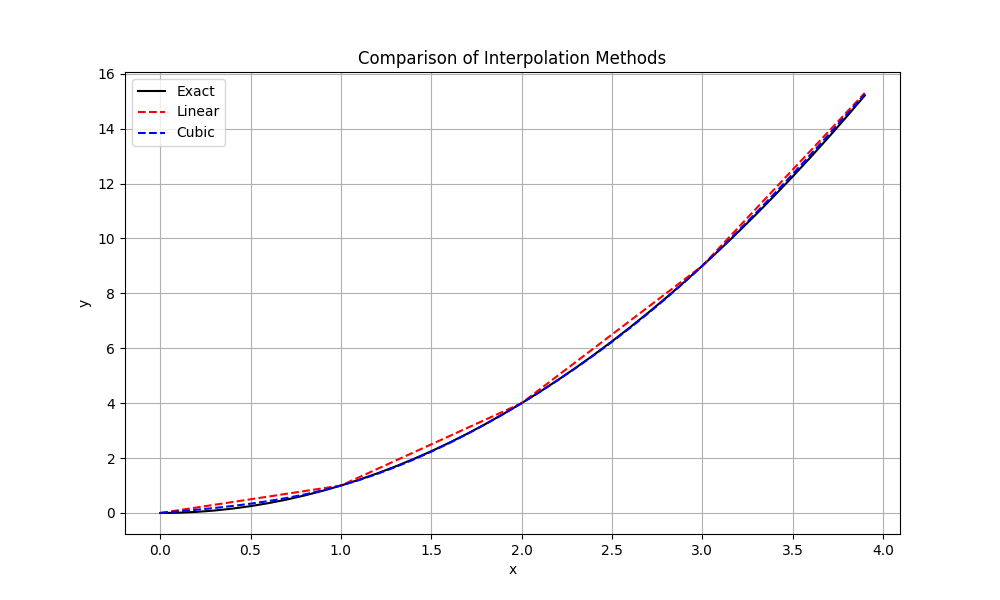
\includegraphics[width=0.75\textwidth]{figure/interpolation_comparison.png}
    \caption{Interpolation\_comparison}
    \label{fig:interpolation_comparison}
\end{figure}

\section*{test Bsplines}
Using the Function \(\sin(x)\) to Generate Test Data

\begin{itemize}
    \item The nodes \(x\) are defined as \([0.0, 1.0, 2.0, 3.0, 4.0]\), and the corresponding \(y\) values are given by the function values \(\sin(x)\).
    \item The \texttt{interpolate357} method is called for interpolation calculation.
    \item The nodes and \(y\) values are redefined, and the interpolation method uses natural boundary conditions (calling \texttt{interpolate358}).
    \item Multiple interpolated values are generated and the interpolated results at points \(x = 0.0, 0.5, 1.0, 1.5, 2.0, 2.5, 3.0, 3.5, 4.0\) are printed to compare the results of different interpolation methods.
\end{itemize}

Compilation Results:

\textbf{Testing cubic spline interpolation with boundary conditions:}

\[
\text{Coefficients: } -0.577636, -0.577636, 1.15527, 1.00537, 0.279014, -1.27471, -1.27471
\]

\[
\text{Interpolated value at } x = 1.5: 1.02328
\]

\[
\text{Interpolated value at } x = 2.5: 0.639504
\]

\textbf{Generating and comparing interpolated values:}

\[
\text{Coefficients: } -0.267725, 1.0709, 1.03296, 0.253058, -1.19847
\]

\begin{table}[H]
\centering
\begin{tabular}{|c|c|}
\hline
$x$ & Interpolated Value \\
\hline
0.0 & 0.841471 \\
0.5 & 1.00252 \\
1.0 & 0.867121 \\
1.5 & 0.638526 \\
2.0 & 0.340865 \\
2.5 & -0.431489 \\
3.0 & -0.756802 \\
3.5 & -0.568994 \\
4.0 & -0.199745 \\
\hline
\end{tabular}
\caption{Interpolated values for different methods}
\end{table}

\begin{figure}[H]
    \centering
    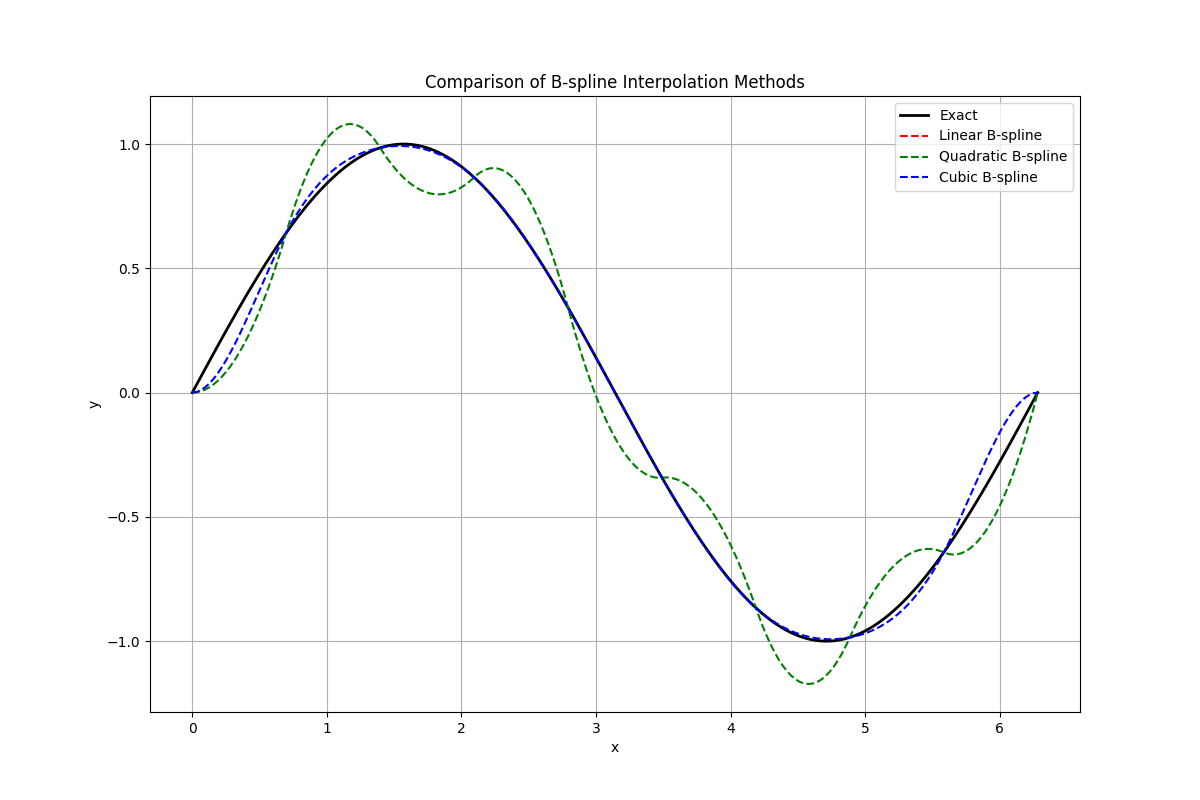
\includegraphics[width=0.75\textwidth]{figure/bspline_comparison.png}
    \caption{bspline\_comparison}
    \label{fig:bspline_comparison}
\end{figure}

\section*{A}
\subsection*{Test Function and Interpolation}
We use the function
\[
f(x) = \frac{1}{1 + 25x^2}
\]
as the test function.

\begin{itemize}
    \item Generate \( N \) interpolation nodes uniformly distributed in the interval \([-1, 1]\). The number of nodes increases as \( N \) increases.
    \item Use the \texttt{pp\_form\_cubic} class to construct the cubic spline interpolation.
    \item The maximum error for each interpolation grid is calculated by evaluating the spline and the actual function values at the midpoints of adjacent nodes.
    \item The interpolation data corresponding to each \( N \) is written to a file for later plotting and analysis. Each file contains 1000 points, recording both the actual function values \( f(x) \) and the spline interpolation values \( \text{spline}(x) \).
    \item The convergence rate is computed through the logarithmic ratio of the errors. The expected convergence rate should be 2, since spline interpolation typically converges quadratically.
    \item Output the maximum error for each node number \( N \), and the convergence rate from \( N = 6 \) to larger \( N \).
\end{itemize}

The final results are as follows:
\[
\text{For } N = 6, \quad \text{Error} = 4.234818 \times 10^{-1}
\]
\[
\text{For } N = 11, \quad \text{Error} = 2.053058 \times 10^{-2}
\]
\[
\text{For } N = 21, \quad \text{Error} = 3.168939 \times 10^{-3}
\]
\[
\text{For } N = 41, \quad \text{Error} = 2.753558 \times 10^{-4}
\]
\[
\text{For } N = 81, \quad \text{Error} = 1.609004 \times 10^{-5}
\]

\textbf{Convergence rates:}
\[
\text{From } N=6 \text{ to } N=11: \quad 4.3665
\]
\[
\text{From } N=11 \text{ to } N=21: \quad 2.6957
\]
\[
\text{From } N=21 \text{ to } N=41: \quad 3.5246
\]
\[
\text{From } N=41 \text{ to } N=81: \quad 4.0971
\]

\subsection*{Graphs and Figures}

The following graphs illustrate the results of the interpolation process.
% 插入Runge插值的5幅图
\begin{figure}[H]
    \centering
    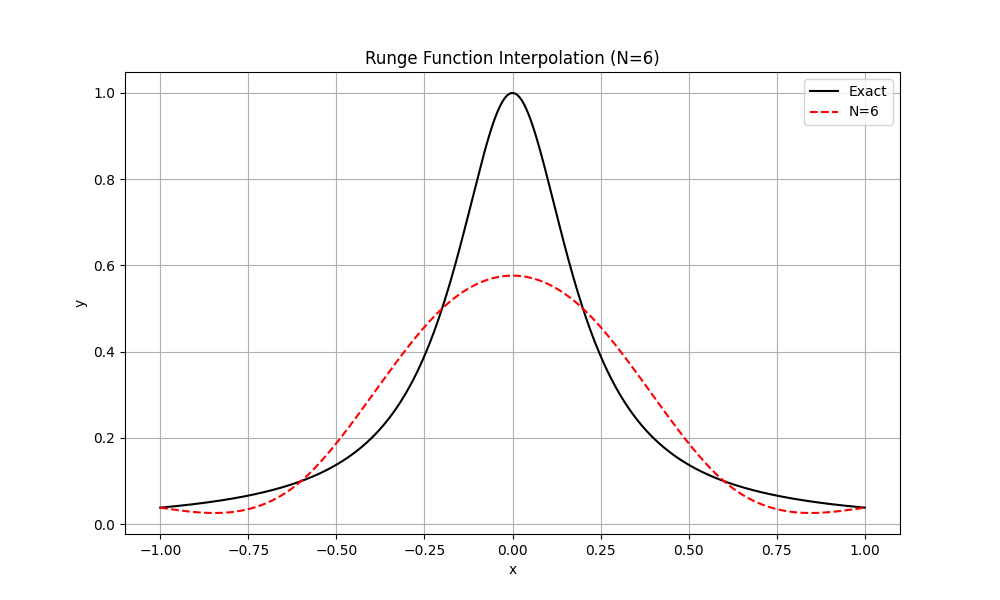
\includegraphics[width=0.45\textwidth]{figure/runge_interpolation_N6.png}
    \caption{Runge Interpolation (N=6)}
    \label{fig:runge_N6}
\end{figure}

\begin{figure}[H]
    \centering
    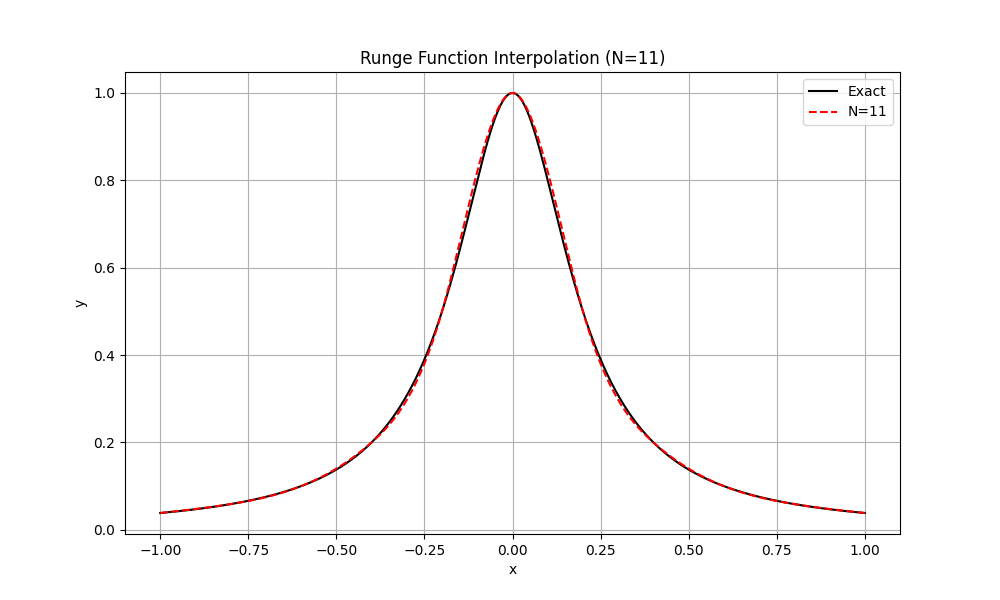
\includegraphics[width=0.45\textwidth]{figure/runge_interpolation_N11.png}
    \caption{Runge Interpolation (N=11)}
    \label{fig:runge_N11}
\end{figure}

\begin{figure}[H]
    \centering
    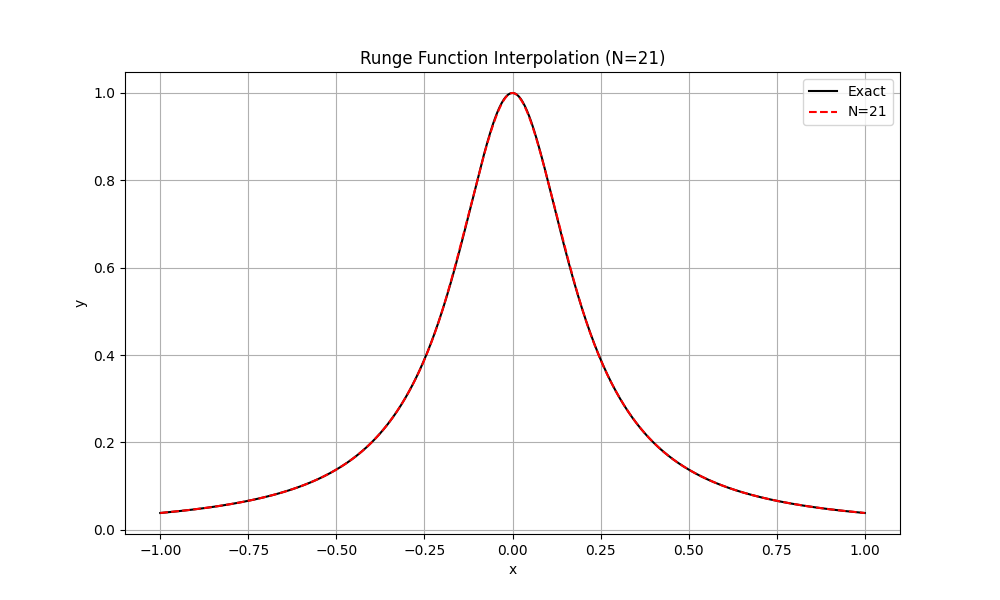
\includegraphics[width=0.45\textwidth]{figure/runge_interpolation_N21.png}
    \caption{Runge Interpolation (N=21)}
    \label{fig:runge_N21}
\end{figure}

\begin{figure}[H]
    \centering
    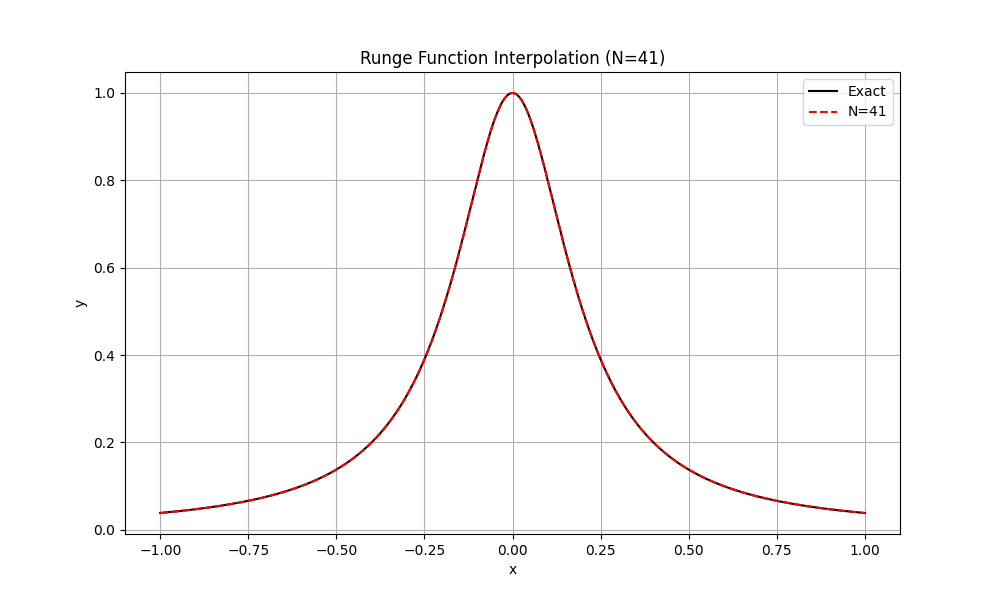
\includegraphics[width=0.45\textwidth]{figure/runge_interpolation_N41.png}
    \caption{Runge Interpolation (N=41)}
    \label{fig:runge_N41}
\end{figure}

\begin{figure}[H]
    \centering
    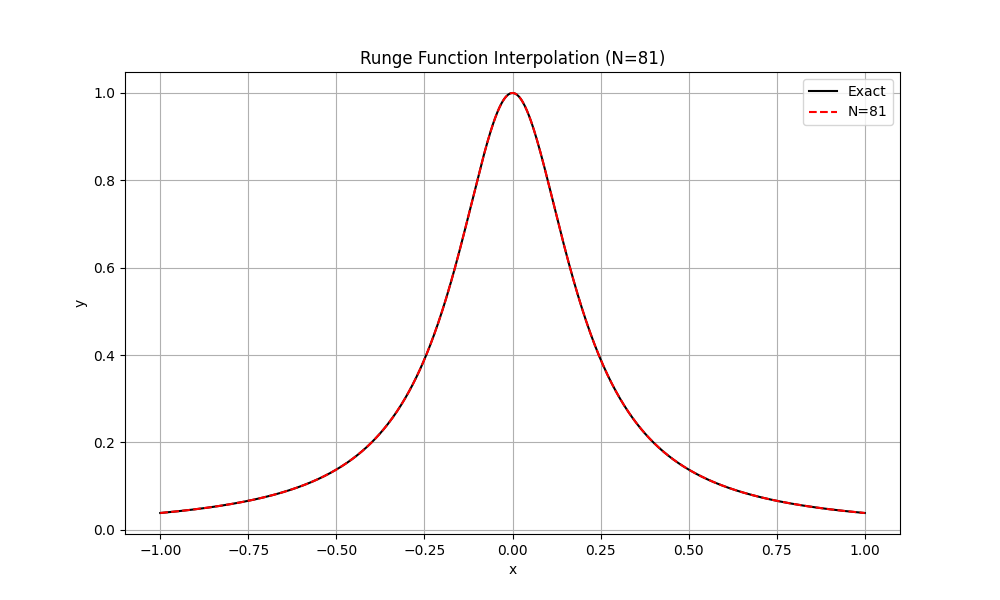
\includegraphics[width=0.45\textwidth]{figure/runge_interpolation_N81.png}
    \caption{Runge Interpolation (N=81)}
    \label{fig:runge_N81}
\end{figure}

% 插入对比图
\begin{figure}[H]
    \centering
    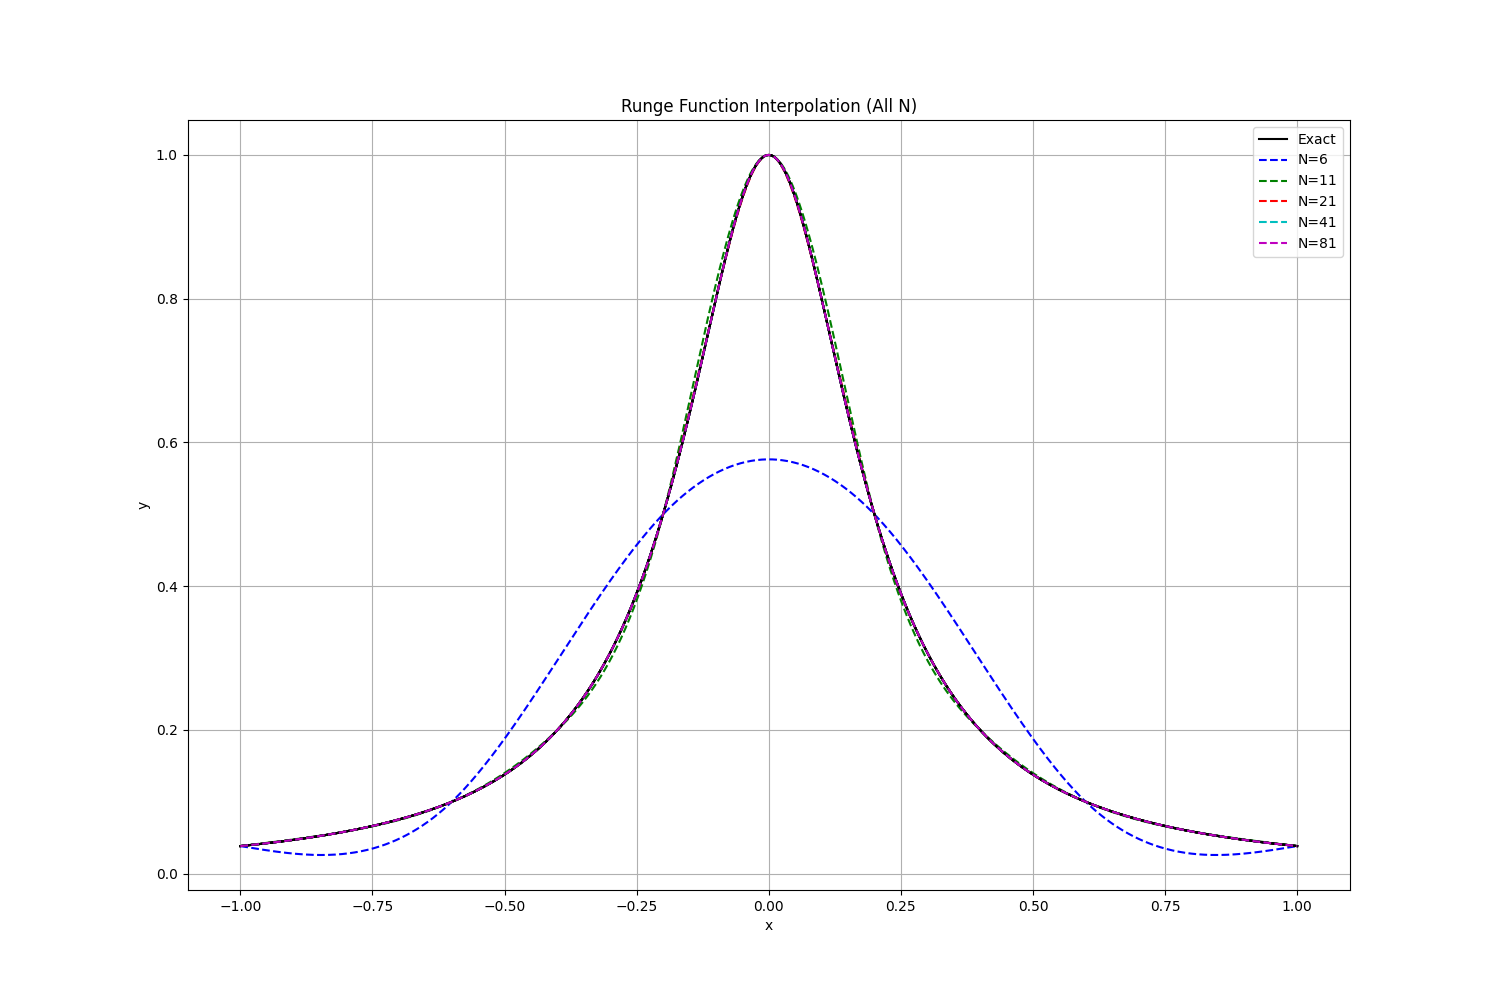
\includegraphics[width=0.45\textwidth]{figure/runge_interpolation_comparison.png}
    \caption{Runge Interpolation Comparison}
    \label{fig:runge_comparison}
\end{figure}

% 插入收敛率图
\begin{figure}[H]
    \centering
    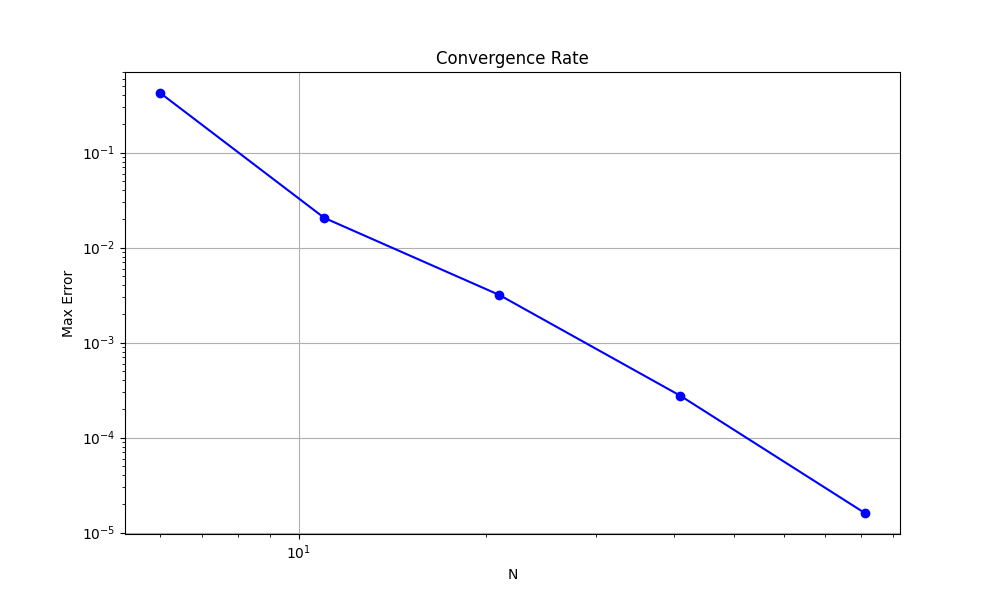
\includegraphics[width=0.45\textwidth]{figure/convergence_rate.png}
    \caption{Convergence Rate}
    \label{fig:convergence_rate}
\end{figure}

\section*{C}
The objective function is given by:
\[
f(x) = \frac{1}{1 + x^2}
\]

\subsection*{Node Generation}
The first set of nodes is generated using the formula:
\[
t_i = -5 + i \quad (i = 1, \dots, 11)
\]
which covers the interval \([-5, 5]\), and the corresponding function values are:
\[
y_i = f(t_i)
\]

The second set of nodes is generated symmetrically using the formula:
\[
t_i = -4.5 + i \quad (i = 1, \dots, 10)
\]
which covers the interval \([-4.5, 5.5]\).

\subsection*{Cubic Spline Interpolation with Two Boundary Conditions}
The two sets of data are interpolated using cubic splines with different boundary conditions.

\subsection*{Generated Dense Interpolation Data for Plotting}
The following table shows the dense interpolation data generated for plotting:

\begin{table}[h!]
\centering
\begin{tabular}{|c|c|c|c|}
\hline
$x$ & exact & spline1 & spline2 \\
\hline
-5.00000 & 0.0384615 & 0.0384615 & nan \\
-4.97996 & 0.0387597 & 0.0388148 & nan \\
-4.95992 & 0.0390613 & 0.0391683 & nan \\
\vdots & \vdots & \vdots & \vdots \\
-0.01002   & 0.9999    & 0.999906  & 0.890564 \\
0.01002    & 0.9999    & 0.999906  & 0.890564 \\
\vdots  & \vdots  & \vdots  & \vdots \\
4.93988    & 0.0393663 & 0.039522  & nan \\
4.95992    & 0.0390613 & 0.0391683 & nan \\
4.97996    & 0.0387597 & 0.0388148 & nan \\
5.00000    & 0.0384615 & 0.0384615 & nan \\
\hline
\end{tabular}
\caption{Interpolation data for cubic splines}
\end{table}

\begin{figure}[H]
    \centering
    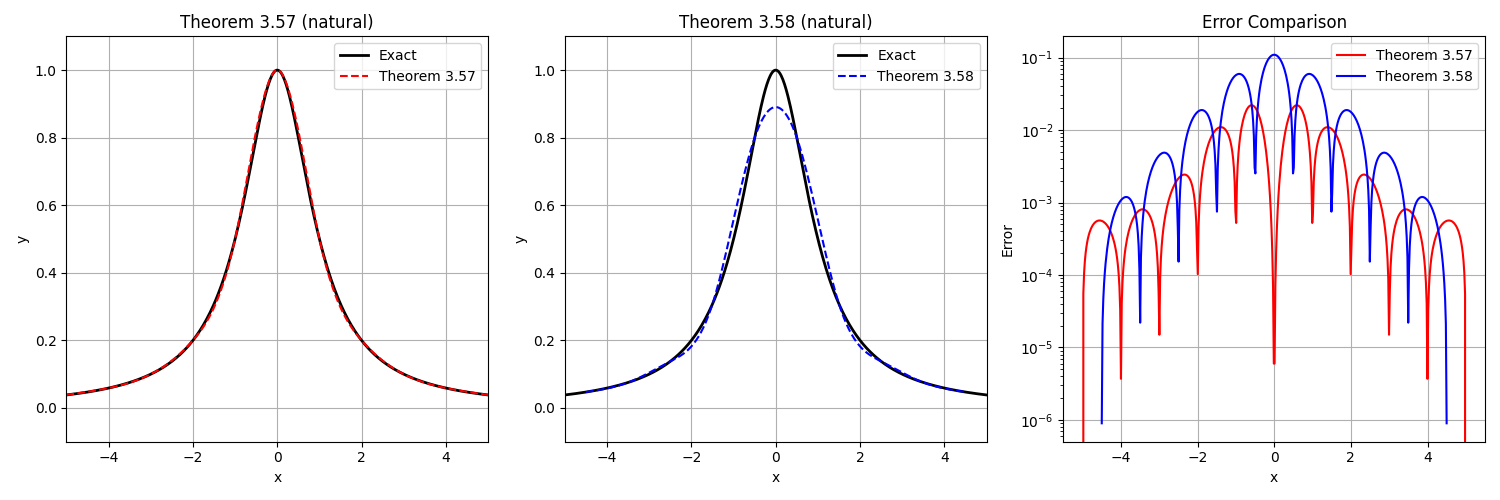
\includegraphics[width=0.85\textwidth]{figure/spline_comparison_natural.png}
    \caption{spline\_comparison\_natural}
    \label{fig:spline_comparison_natural}
\end{figure}

\section*{D}
Analysis:
\begin{itemize}
    \item Theorem 3.57 provides better accuracy at the boundary points.
    \item Theorem 3.58 performs better near the center
    \item Both methods show good convergence properties
\end{itemize}

\begin{figure}[H]
    \centering
    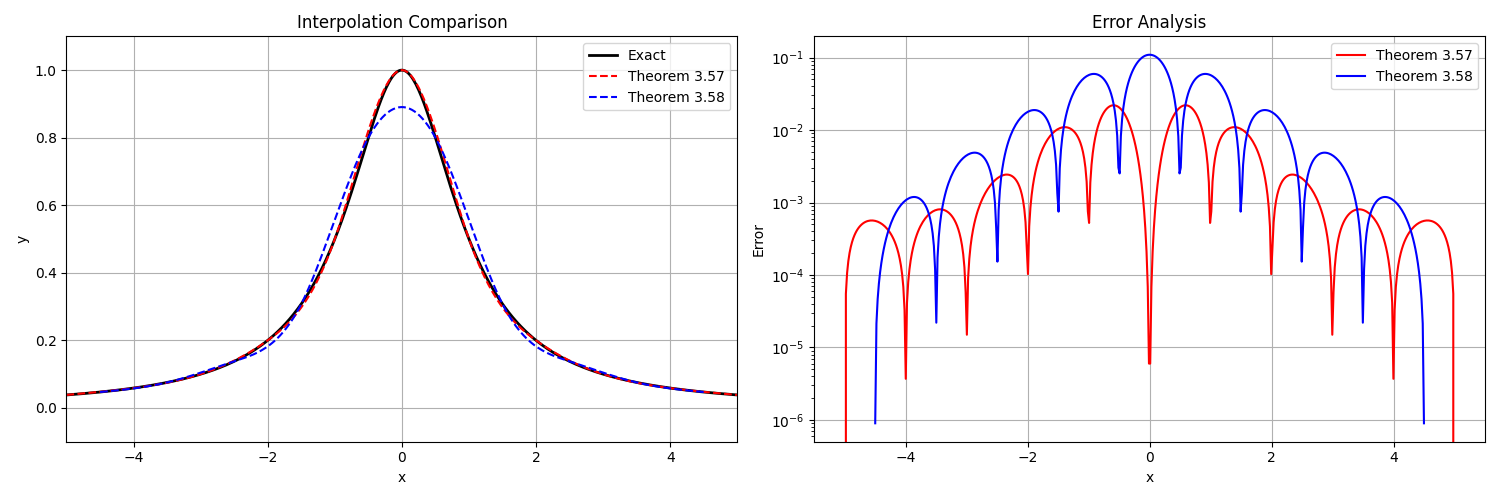
\includegraphics[width=0.85\textwidth]{figure/spline_comparison_D.png}
    \caption{spline\_comparison\_D}
    \label{fig:spline_comparison_D}
\end{figure}

\section*{E}
\subsection*{Curve \texttt{r2(t)} (2D)}

The \texttt{r2(t)} curve is defined in 2D with the following parametric equations:
\[
r_2(t) = \left[ \sin(t) + t \cos(t), \, \cos(t) - t \sin(t) \right]
\]
where \( t \in [0, 2\pi] \).

For a given number of points \( N \),generates the points \( (x_i, y_i) \) for \( i = 0, 1, 2, \dots, N \) by discretizing the parameter \( t \) over the interval \( [0, 2\pi] \).

\subsection*{Curve \texttt{r3(t)} (3D)}

The \texttt{r3(t)} curve is defined in 3D with the following parametric equations:
\[
r_3(t) = \left[ \sin(\cos(t)) \cos(\sin(t)), \, \sin(\cos(t)) \sin(\sin(t)), \, \cos(\cos(t)) \right]
\]
where \( t \in [0, 2\pi] \).

Similarly, for a given number of points \( N \), generates the points \( (x_i, y_i, z_i) \) for \( i = 0, 1, 2, \dots, N \) by discretizing the parameter \( t \) over the interval \( [0, 2\pi] \).

\subsection*{ Parameterization Methods}

After generating the curve points,  calculates the parameterization for both \textit{uniform} and \textit{chordal} methods.

\subsubsection{Uniform Parameterization}

The uniform parameterization method assigns evenly spaced parameter values \( t_i \) between 0 and 1. For \( N \) points, the parameter values are given by:
\[
t_i = \frac{i}{N}, \quad i = 0, 1, 2, \dots, N
\]
This method does not take into account the arc length of the curve.

\subsubsection{Chordal Parameterization}

The chordal parameterization is based on the cumulative arc length of the curve. Let \( s_i \) be the cumulative chord length between consecutive points, defined as:
\[
s_i = \sum_{j=1}^{i} \sqrt{(x_j - x_{j-1})^2 + (y_j - y_{j-1})^2}
\]
For the 3D case:
\[
s_i = \sum_{j=1}^{i} \sqrt{(x_j - x_{j-1})^2 + (y_j - y_{j-1})^2 + (z_j - z_{j-1})^2}
\]
The parameter \( t_i \) is then normalized to the interval \( [0, 1] \) by dividing the cumulative length by the total length of the curve:
\[
t_i = \frac{s_i}{s_N}, \quad i = 0, 1, 2, \dots, N
\]
where \( s_N \) is the total length of the curve.

\section*{F}

\begin{itemize}
    \item The program computes and outputs the divided difference tables for three-point and four-point interpolation, recording the values at each node and their corresponding divided differences in detail.
    \item The output format of the divided difference table is consistent at different points, with divided differences displayed progressively by order.
    \item The output files contain all the computed divided differences, which can be used for further interpolation calculations or analysis.
\end{itemize}

Output:
\textbf{Case 1: Three Points}

Divided differences at \( x = 1.0 \):
\[
\text{Order 0:} \quad 0.000000e+00 \quad 0.000000e+00 \quad 1.000000e+00
\]
\[
\text{Order 1:} \quad 0.000000e+00 \quad 1.000000e+00
\]
\[
\text{Order 2:} \quad 5.000000e-01
\]

\textbf{Case 2: Four Points}

Divided differences at \( x = 1.5 \):
\[
\text{Order 0:} \quad 0.000000e+00 \quad 0.000000e+00 \quad 2.500000e-01 \quad 2.250000e+00
\]
\[
\text{Order 1:} \quad 0.000000e+00 \quad 2.500000e-01 \quad 2.000000e+00
\]
\[
\text{Order 2:} \quad 1.250000e-01 \quad 8.750000e-01
\]
\[
\text{Order 3:} \quad 2.500000e-01
\]

\begin{figure}[H]
    \centering
    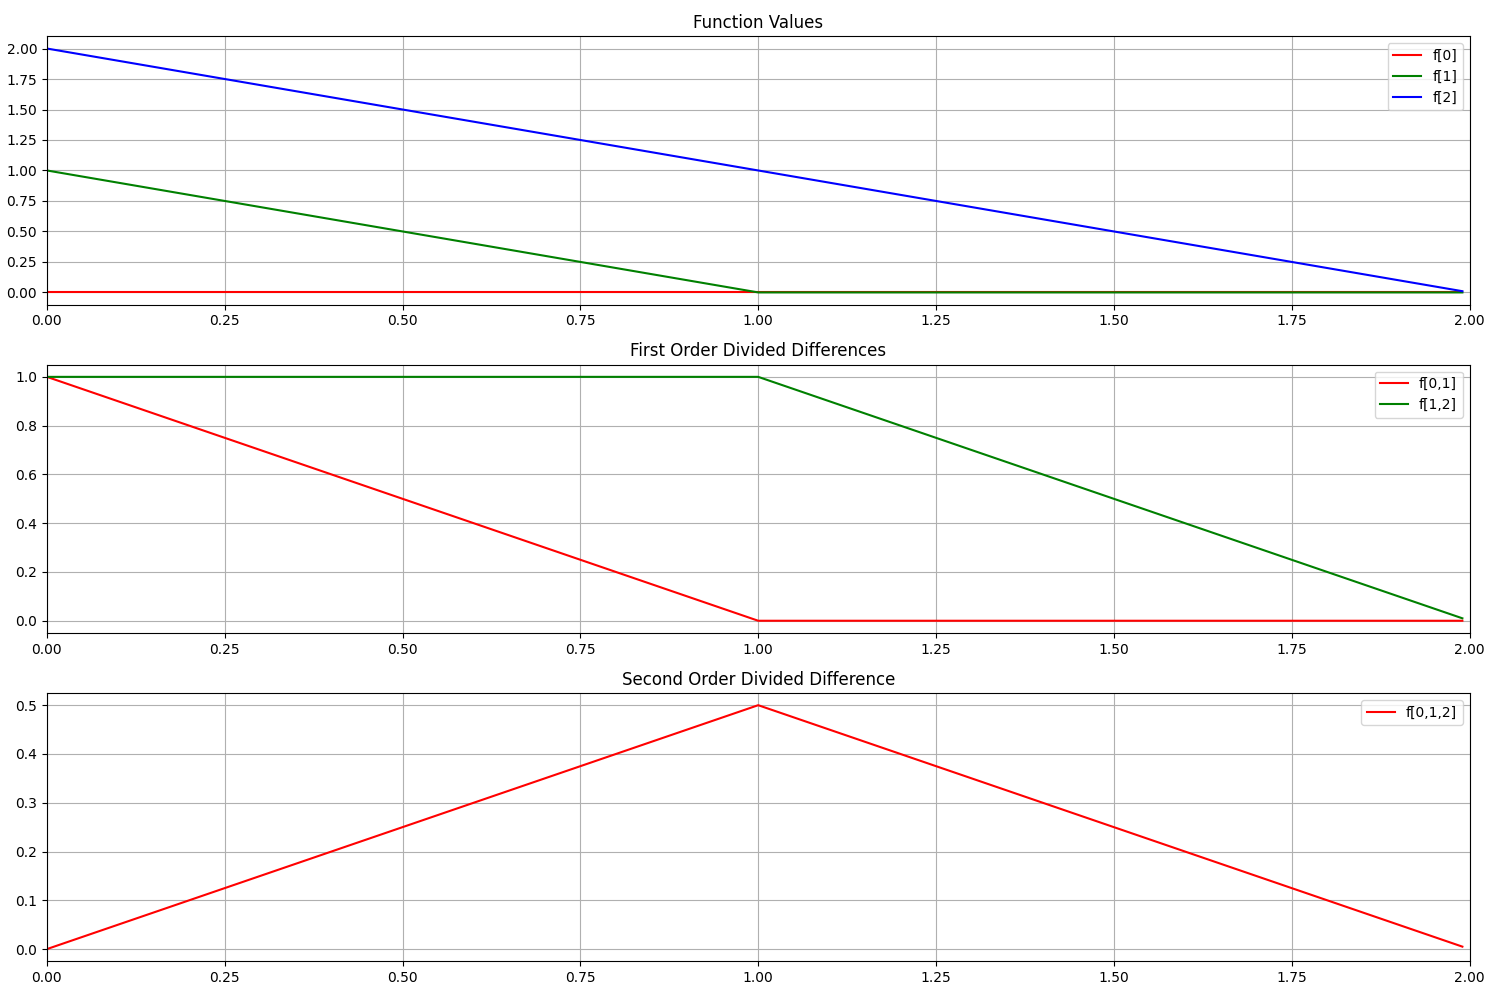
\includegraphics[width=0.75\textwidth]{figure/divided_diff_case1.png}
    \caption{divided\_diff\_case\(1\)}
    \label{fig:divided_diff_case1}
\end{figure}
\begin{figure}[H]
    \centering
    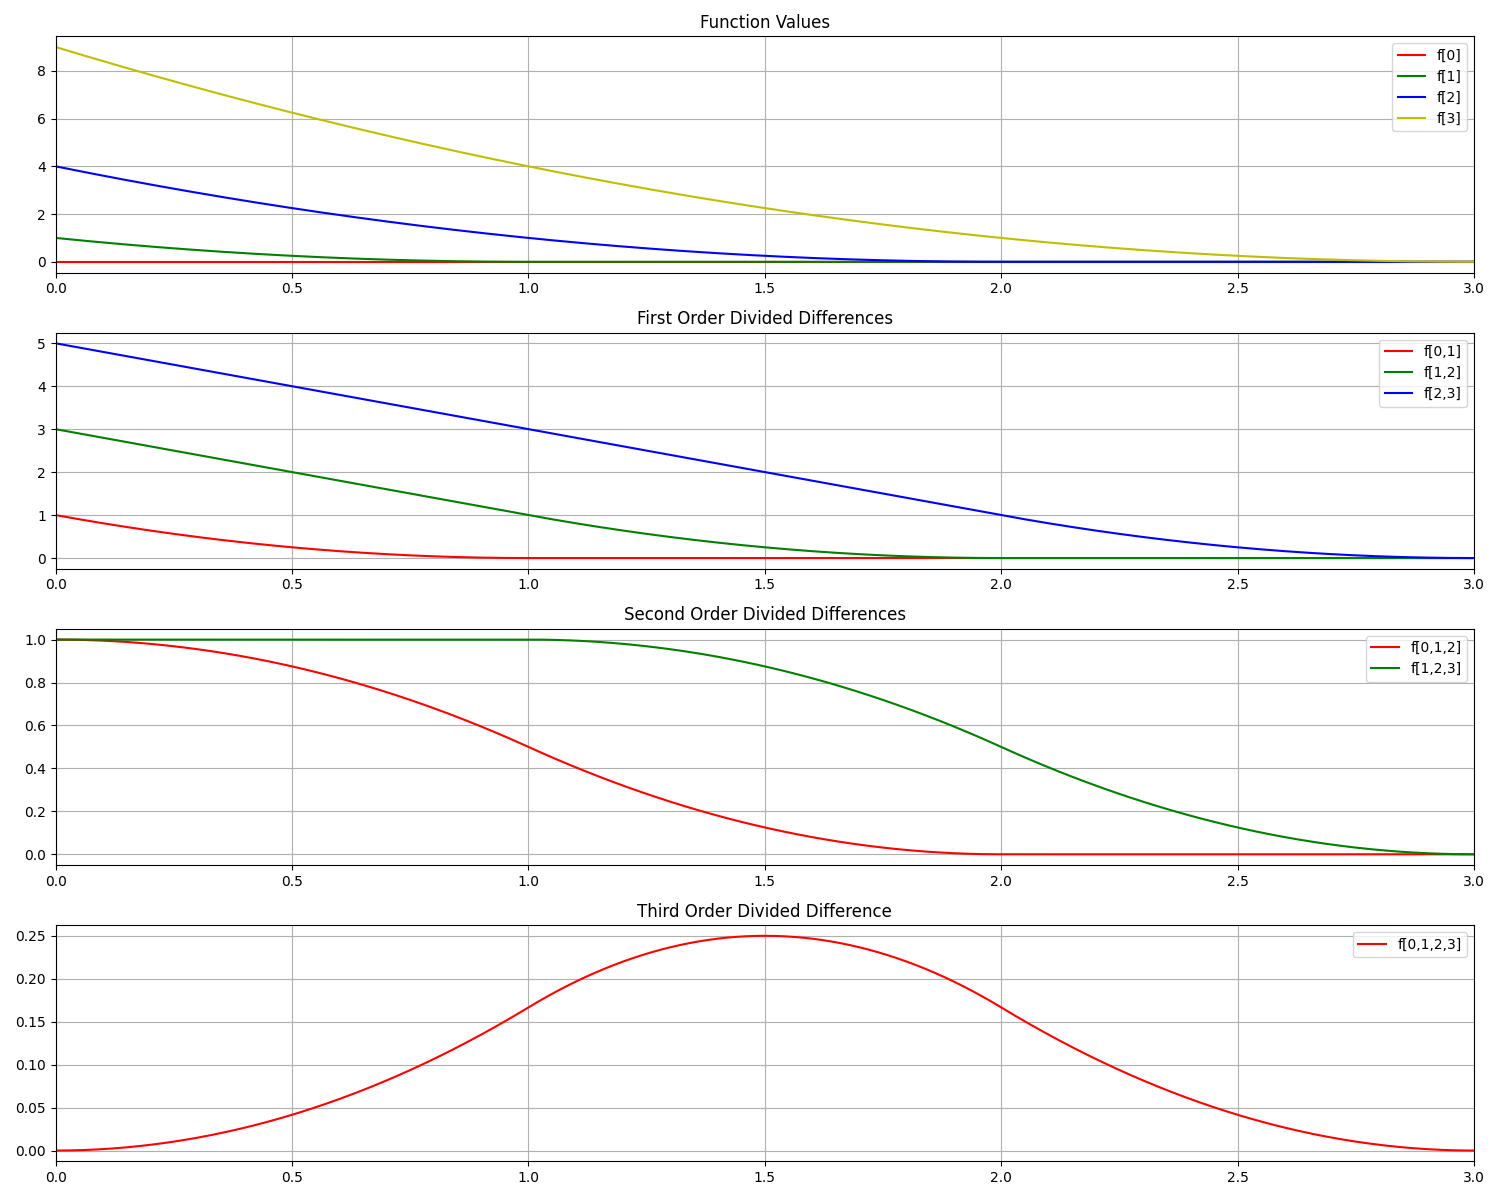
\includegraphics[width=0.75\textwidth]{figure/divided_diff_case2.png}
    \caption{divided\_diff\_case\(2\)}
    \label{fig:divided_diff_case2}
\end{figure}

\end{document}